\subsection{Data}
We use the Shenzhen taxicab GPS subset from the Urban Data Release V2 / UrbanCPS dataset \citep{zhang2015urbancps}, which provides multi-source urban mobility logs (CDR, smartcard, taxi/bus/truck GPS) for academic research. In this project we focus on the taxi GPS modality; each record contains anonymized taxi ID, timestamp, latitude, longitude, occupancy status, and speed. For privacy, identifiable IDs are replaced by serial numbers and date information may be obfuscated in the public release.

We preprocess the taxi trajectories into a grid-based representation. The spatial domain is rasterized into a $400 \times 800$ grid with a geographic bounding box (latitude $[22.45, 22.85]$, longitude $[113.75, 114.65]$). Each trajectory stores positions in grid coordinates $[y, x]$ along with timestamps.

\paragraph{dt-fixed resampling (Phase B).}
To make temporal semantics explicit and enable physically meaningful macroscopic metrics (e.g., MSD as a function of real time), we resample trajectories to a fixed interval $\Delta t = 30$s. Trajectory segments with gaps exceeding $300$s are dropped, and short segments are filtered. After resampling, the split sizes are:
train = 97,222, val = 21,103, test = 21,309 trajectories.

\paragraph{Leakage-free strict products.}
All normalization statistics and the navigation field are computed using \textbf{train split only}. The processed artifacts include:
\begin{itemize}
  \item \texttt{data\_stats.json}: train-only normalization (pos bounds, vel mean/std) and metadata hashes.
  \item \texttt{nav\_field.npz}: train-only navigation field (local mean-flow prior) with recorded source split.
\end{itemize}
This strict contract prevents information leakage from validation/test into the physics prior.

\subsection{Problem Setup}
We consider window-based forecasting with observation length $\texttt{obs\_len}=8$ and prediction length $\texttt{pred\_len}=12$ (i.e., 4 minutes of history and 6 minutes of future at $\Delta t = 30$s). The model outputs future \texttt{vel}, where \texttt{vel} is defined as \emph{step displacement} in grid units per step. Under fixed $\Delta t$, physical velocity is proportional to this displacement.

The task is \textbf{KnownDestination}: destination $d$ is provided at inference time as part of the conditioning (OD-conditioned generation).

\subsection{Models}
\paragraph{Deterministic baseline (L2 regression).}
We implement a sequence regression baseline that predicts a single future trajectory by minimizing L2 loss. This model is deterministic ($K=1$) and serves as a strong mean-accuracy reference.

\paragraph{Conditional diffusion trajectory generator.}
We model the conditional distribution of future velocity sequences using a denoising diffusion framework \citep{ho2020ddpm}. Given observed history and OD context, the model samples $K$ future trajectories via a reverse diffusion process.

\paragraph{Physics-conditioned diffusion (nav\_field).}
We extend diffusion by injecting a navigation field patch cropped around the current location. The nav\_field is a train-only, grid-aligned mean-flow prior estimated from historical trajectories. This provides a local directional bias while keeping the representation grid-based (v1 does not perform road-level map matching).

\begin{figure}[t]
  \centering
  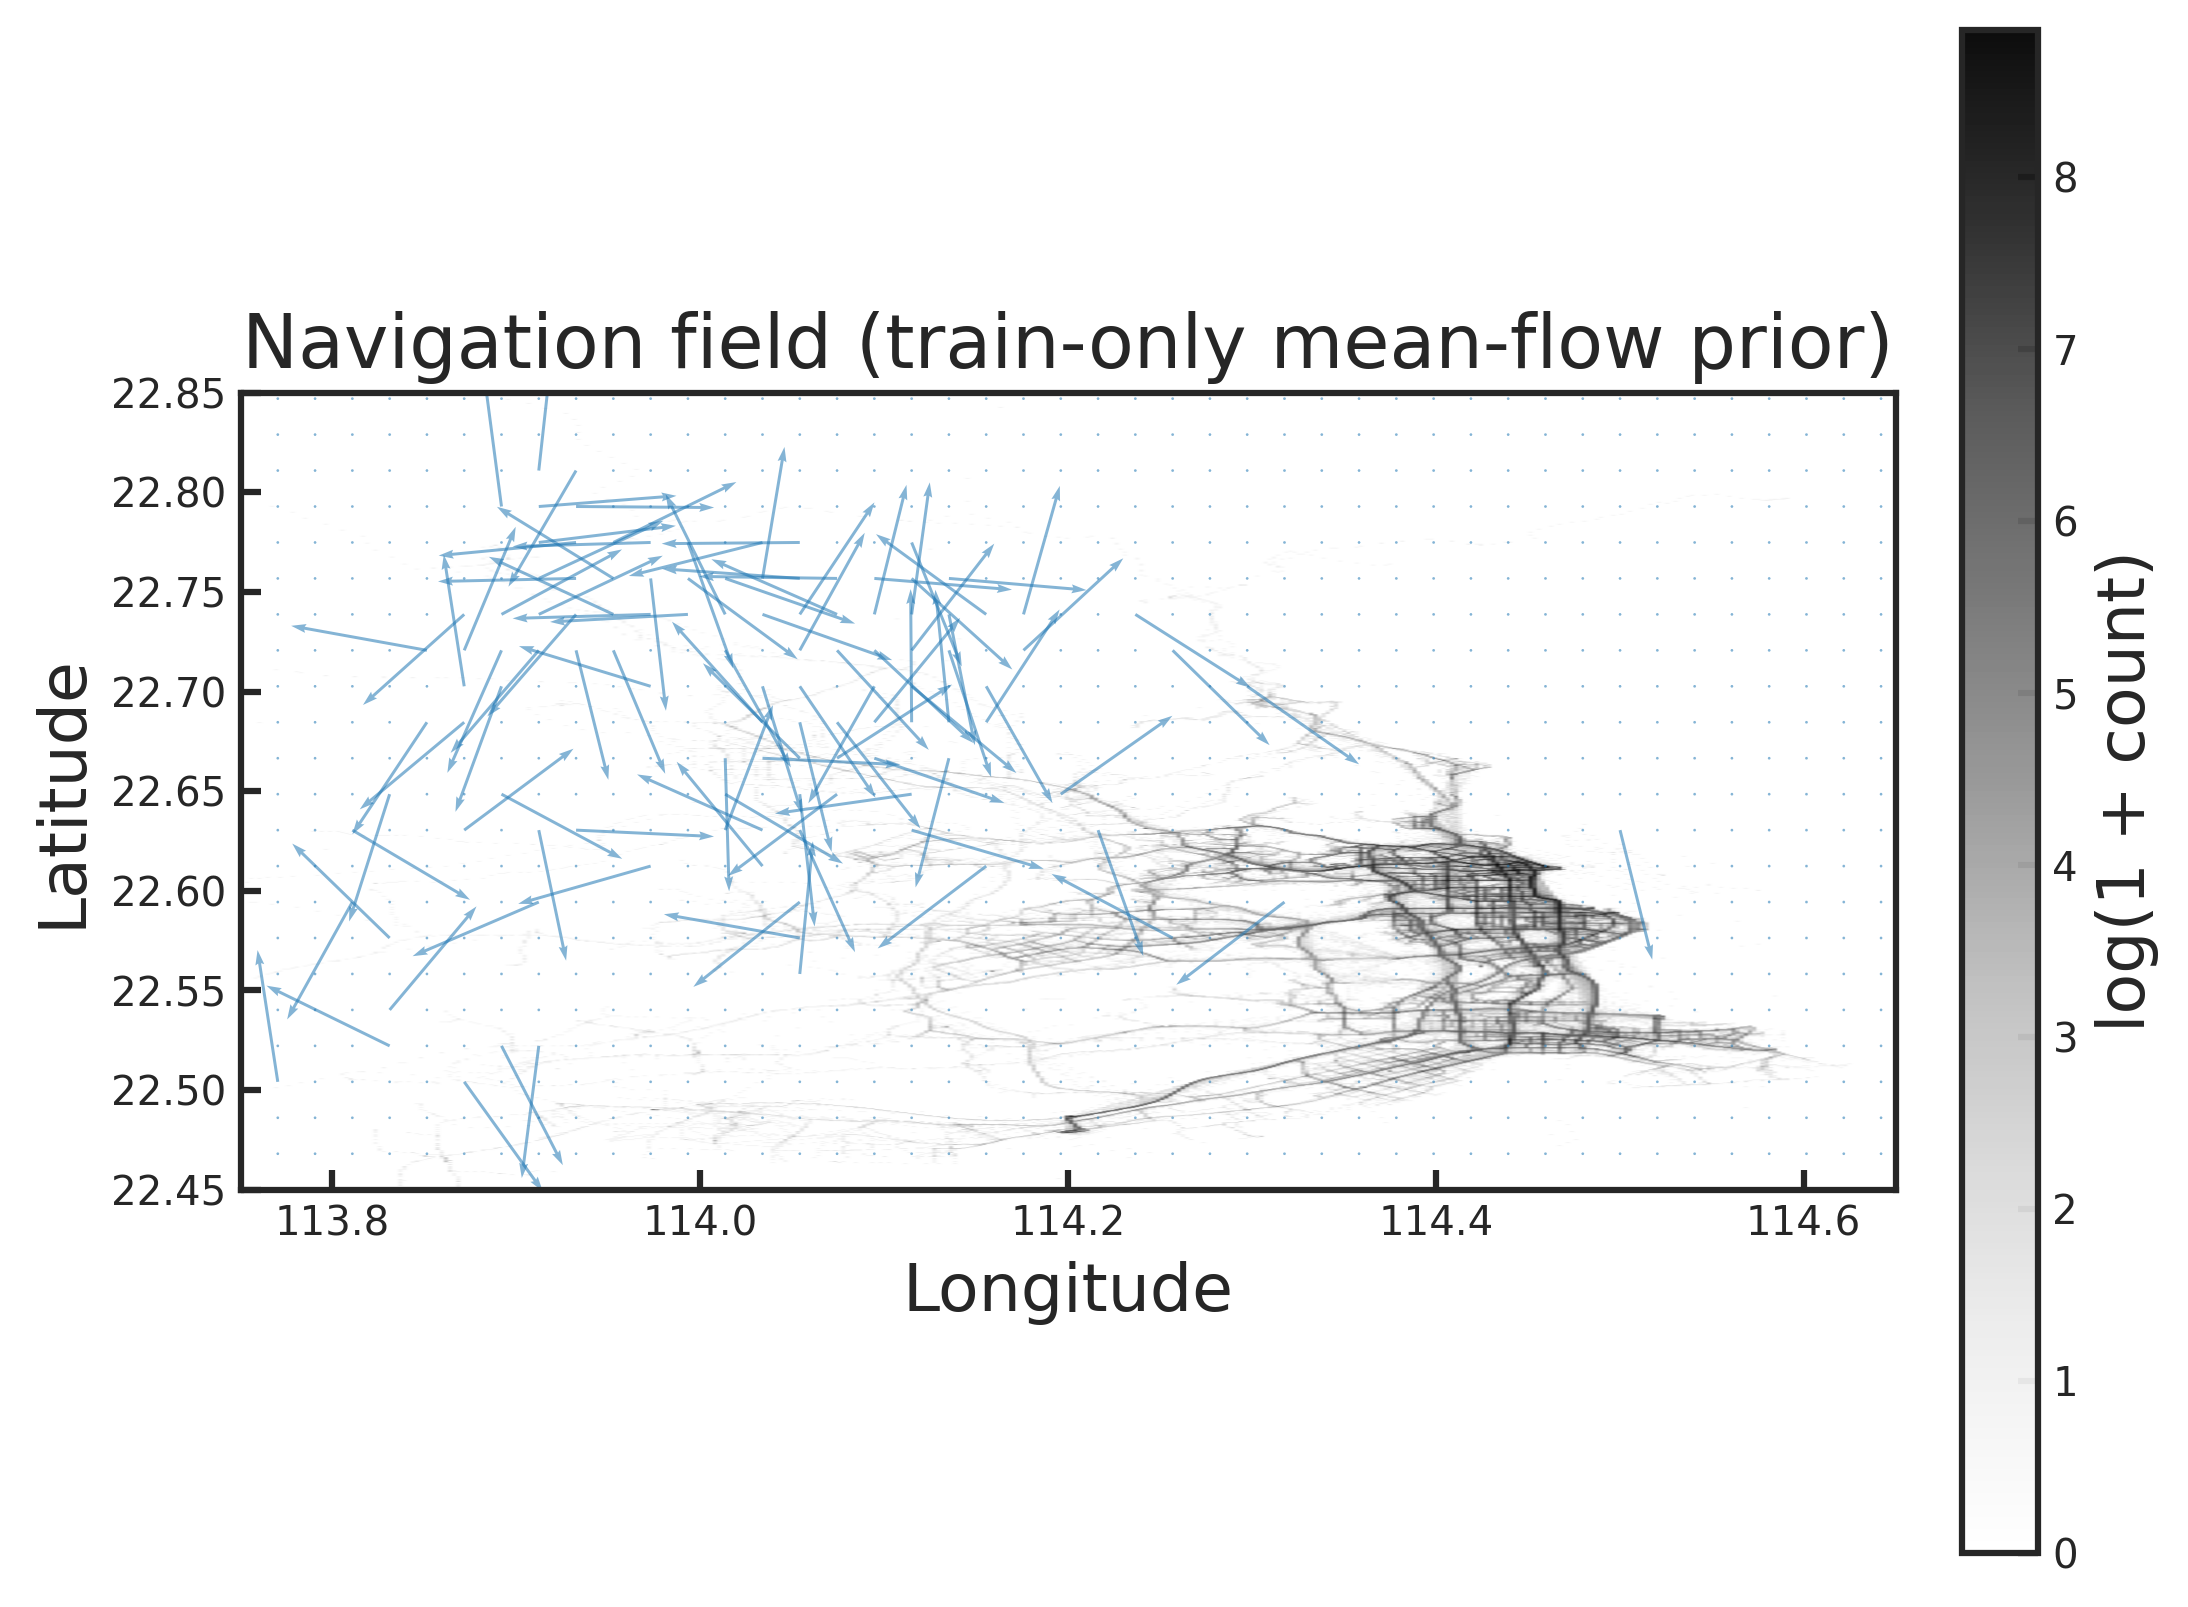
\includegraphics[width=0.90\linewidth]{figures/fig_geo_nav_field.png}
  \caption{Train-only navigation field visualized in geographic space (mean-flow prior; bbox linear mapping for display).}
  \label{fig:navfield}
\end{figure}

Figure~\ref{fig:navfield} provides an intuitive view of this prior: dense regions correspond to frequent historical observations, and arrows indicate the local mean-flow direction estimated from the training split.

\subsection{Training Objective}
The core objective is the diffusion loss (noise-prediction MSE). We additionally explore training-time \emph{macroscopic} constraints (e.g., end-to-end displacement error) to improve low-frequency structure and directional persistence. To avoid shortcut solutions at highly noisy diffusion timesteps, macro losses can be gated to apply only at early timesteps where the signal-to-noise ratio is higher (hard thresholding).

\subsection{Evaluation Protocol}
We evaluate on the test split using:
\begin{itemize}
  \item \textbf{Micro metrics}: ADE/FDE with mean/std across $K$ samples and best-of-$K$ (oracle) as a coverage upper bound; Fr\'echet distance and DTW as distribution-aware measures.
  \item \textbf{Macro metrics}: MSD curve (as a function of lag $\tau = k\Delta t$) and Rog, reported for both predictions and ground truth.
\end{itemize}
For fair comparison, deterministic baselines are evaluated with $K=1$, while generative models use $K=20$ by default.

\subsection{Geographic-space visualization (for urban interpretation)}
Although models operate in grid space, we map grid coordinates back to latitude/longitude via a linear bbox projection for visualization. This enables ``map-like'' plots (trajectory overlays and spatial density maps) that help interpret how generated mobility patterns distribute over the city. We emphasize that this is an approximate visualization for v1 and does not enforce road-network constraints.
